\documentclass[t]{beamer}

% Load general definitions
% Preamble file - general definitions, package loading, etc.

%=================================
% Load packages
\usepackage{amssymb,amsmath}
\usepackage{graphicx}
\usepackage{url}
\usepackage{tikz}
\usetikzlibrary{mindmap,trees,arrows}
\usepackage{fancyvrb}
\usepackage[portuguese]{babel} 
\usepackage[utf8]{inputenc}
\usepackage{subfigure}
\usepackage{times}
\usepackage[T1]{fontenc}
\usepackage{cancel}
\usepackage{color}
\usepackage{listings}
\usepackage[document]{ragged2e}

%=================================
% Set mode
\mode<presentation>
{
	\usetheme{Madrid}
	\usecolortheme{structure}
	\useoutertheme{infolines}
	\setbeamercovered{invisible}
}

% Get rid of nav bar
\beamertemplatenavigationsymbolsempty

% Insert frame number at bottom of the page.
\usefoottemplate{\hfil\tiny{\color{black!90}\insertframenumber}} 

%=================================
% Define new commands

\newcommand\Real{{\mathbb{R}}}
%\newcommand{\vi}{\vspace{0.6\baselineskip}}
%\newcommand{\goodgap}{\hspace{\subfigtopskip}\hspace{\subfigbottomskip}}


% Equation environments
\newcommand{\beq}{\begin{equation}}
\newcommand{\eq}{\end{equation}}
\newcommand{\beqs}{\begin{equation*}}
\newcommand{\eqs}{\end{equation*}}
\newcommand{\beqn}{\begin{eqnarray}}
\newcommand{\eqn}{\end{eqnarray}}
% Bold variables
\newcommand{\mbf}[1]{\ensuremath{\mathbf{#1}}}
% Itemization
\newcommand{\bitem}{\begin{itemize}}
\newcommand{\eitem}{\end{itemize}}
\newcommand{\spitem}{\vskip 1em\item}
\newcommand{\bitems}{\begin{itemize}\item}
\newcommand{\benums}{\begin{enumerate}\item}
\newcommand{\eenum}{\end{enumerate}}
% color blocks
\newenvironment{colorblock}[2]{%
\setbeamercolor{block title}{#2}
\begin{block}{#1}}{\end{block}}
% Vertical spacing
\newcommand{\vone}{\vskip 1em}
\newcommand{\vhalf}{\vskip .5em}
% Frame environments
\newenvironment{ftst}[3][t]{%
\begin{frame}{environment=ftst,#1}
\frametitle{#2}
\framesubtitle{#3}}{\end{frame}}
\newenvironment{ftstf}[2]{
\begin{frame}[fragile,environment=ftstf]
\frametitle{#1}
\framesubtitle{#2}}{\end{frame}}
% colors
\definecolor{MyGray}{rgb}{0.5,0.5,0.5}
\definecolor{MyDBGray}{rgb}{0.1,0.1,0.4}
\definecolor{darkgreen}{rgb}{0,0.4,0}
\definecolor{black}{rgb}{0,0,0}
\def\defn#1{{\color{red} #1}}
% Footnote
\renewcommand{\thefootnote}{\alph{footnote}}
% Relaxed footnotes
\newcommand{\lfr}[1]{\let\thefootnote\relax\footnote{\tiny #1}}
% Verbatim environment - using FANCYVRB package
\DefineVerbatimEnvironment%
{rcode}{Verbatim}
{fontsize=\scriptsize}
% Verbatim environment - using LISTINGS package
%\lstnewenvironment{rcode} {\lstset{	language = R,
%									basicstyle = \scriptsize\ttfamily,
%									showspaces = false,
%									showstringspaces = false,
%									showtabs = false,
%									keywordstyle = \color{black}\bfseries,
%									commentstyle = \color{darkgreen},
%									numbers = none,
%									otherkeywords={	<-,
%													ggplot,
%													geom_boxplot,
%													facet_grid,
%													shapiro.test,
%													fligner.test,
%													glht,
%													with},
%									deletekeywords={data,
%													model,
%													residuals,
%													c,
%													axis,
%													default,
%													labels,
%													qq.text}}}%
%{}

% Specific definitions
\title[]{Metodologia Científica}
\subtitle[]{Estruturação do trabalho científico}
\author[]{Patrícia Lucas\\{\footnotesize }}
\institute{Bacharelado em Sistemas de Informação \\ IFNMG  - Campus Salinas}
\date{\scriptsize Salinas\\Fevereiro 2021}

\begin{document}

% cover page
\setbeamertemplate{footline}{}
\begin{frame}

\begin{center}
\includegraphics[width=.15\textwidth]{}
\end{center}
  \titlepage
  \begin{tikzpicture}[remember picture,overlay]
  \node[anchor=south east,xshift=-5pt,yshift=5pt] at (current page.south east) {\tiny Versão 1.2021};
  \node[anchor=south west,yshift=0pt] at (current page.south west) {
\includegraphics[width=.25\textwidth]{Logos/salinas_horizontal_jpg.jpg}};
  \end{tikzpicture}  
\end{frame}

% Main slides

\begin{ftst}{Referência}{Metodologia Científica}
\vone
\justifying
\begin{figure}
    \centering
    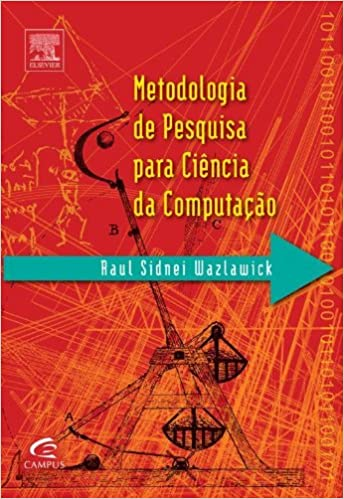
\includegraphics[scale=0.3]{Figuras/ref.jpg}
\end{figure}

WAZLAWICK, R. S. Metodologia de Pesquisa em Ciência da Computação. Rio de Janeiro: Campus, 2009.

\end{ftst}

%=====


\begin{ftst}{A escolha do objetivo da pesquisa}{Estruturação do trabalho científico}
\justifying

O segredo de um trabalho de pesquisa de sucesso consiste em ter um bom objetivo. Uma vez definido o objetivo do trabalho, tudo o mais gravita ao redor dele. 
\vone

\begin{figure}
    \centering
    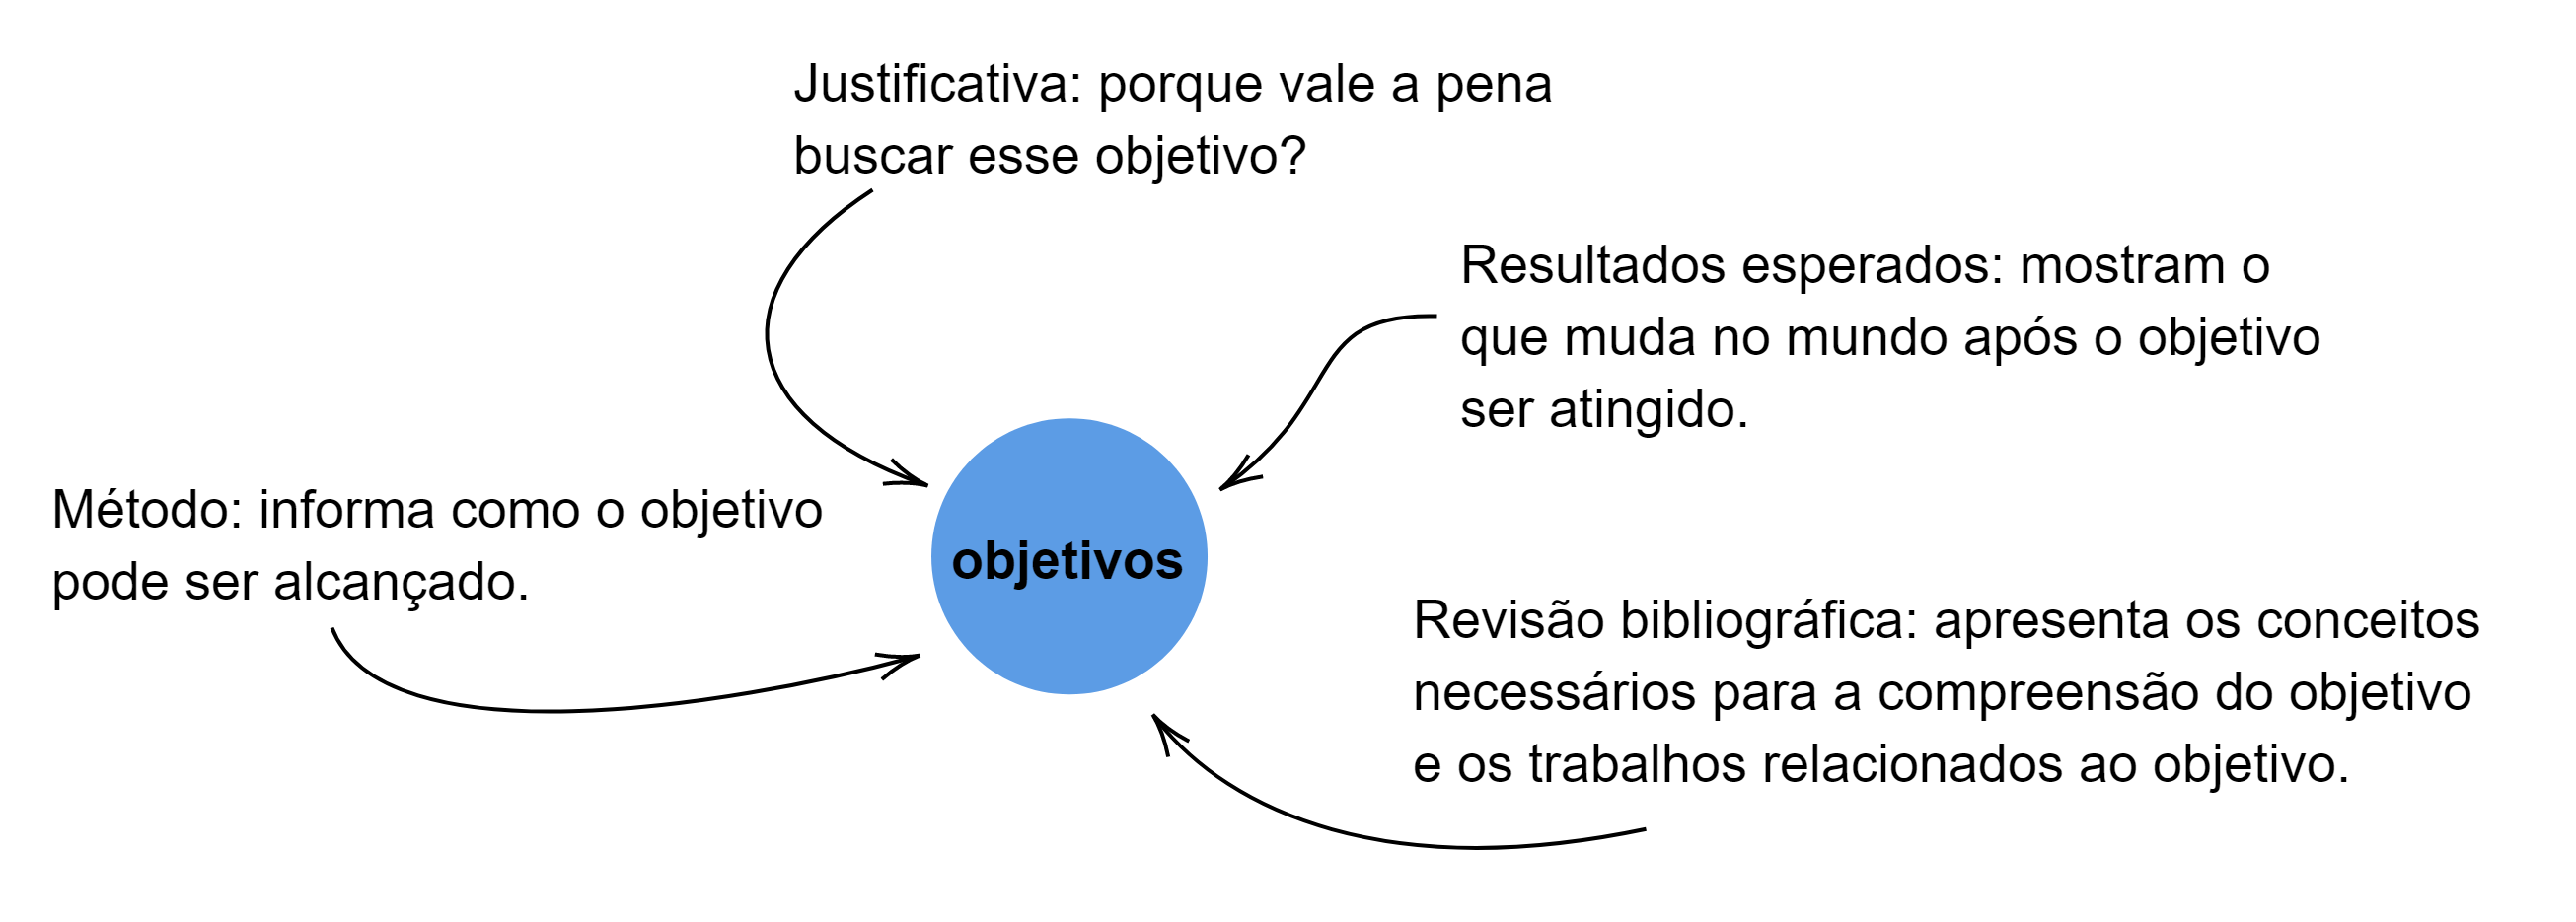
\includegraphics[scale=0.13]{Figuras/03_objetivos.png}
    \label{fig:objetivos}
\end{figure}

\end{ftst}

%=====

\begin{ftst}{A escolha do objetivo da pesquisa}{Estruturação do trabalho científico}
\justifying
\textbf{O caminho para a escolha de um objetivo de pesquisa:}
\vone
\begin{itemize}
    \item Escolher um tema de pesquisa, ou seja, uma área de conhecimento na qual vai trabalhar.
    \item Realizar a revisão bibliográfica. A não ser que o autor já seja especialista na área escolhida, ele vai precisar ler muitos trabalhos já publicados nessa área para saber o que está sendo feito (estado da arte) e o que ainda precisa ser feito (problemas em aberto).
    \item Definir o objetivo de pesquisa. Uma vez feita a revisão bibliográfica, o objetivo de pesquisa possivelmente será fortemente relacionado com um dos problemas em aberto verificados no passo anterior.
\end{itemize}

\end{ftst}

%=====


\begin{ftst}{A escolha do objetivo da pesquisa}{Estruturação do trabalho científico}
\justifying
\textbf{O tema:}
\begin{figure}
    \centering
    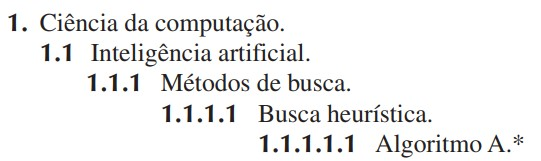
\includegraphics[scale=0.5]{Figuras/03_temas.jpg}
    \label{fig:temas}
\end{figure}
\vone
Quanto mais amplo o tema, maior a quantidade de livros e artigos que terão de ser lidos. Portanto, recomenda-se buscar temas cada vez mais específicos antes de propor um objetivo de pesquisa.

\vone
\textbf{O problema de pesquisa:} uma monografia deve apresentar uma solução para um problema. Dessa forma, um problema deve ser identificado.

\end{ftst}

%=====

\begin{ftst}{A revisão bibliográfica}{Estruturação do trabalho científico}
\justifying
A revisão bibliográfica deve ser muito bem planejada e conduzida.
\vone
Pode-se iniciar a pesquisa com uma leitura de trabalhos mais abrangentes que deem uma visão do todo para depois ir se aprofundando cada vez mais em temas cada vez mais específicos.
\vone
Quando se faz uma pesquisa em que alguma técnica de computação é aplicada a alguma outra área do conhecimento, é necessário fazer a revisão bibliográfica sobre a técnica em si sobre a área de aplicação e, mais do que tudo, sobre as aplicações que já foram tentadas com essa técnica ou com técnicas semelhantes na mesma área ou em áreas equivalentes.


\end{ftst}

%=====

\begin{ftst}{A revisão bibliográfica}{Estruturação do trabalho científico}
\justifying
\textbf{Fichas de leitura:}
\vone
Durante todo o processo de leitura, é fundamental que sejam feitas anotações.
\vone
Conceitos-chave e ideias novas devem ser anotados sempre que forem detectados na leitura. 
\vone
Em geral, inicia-se uma ficha de leitura, seja em papel, seja no computador,
escrevendo a referência bibliográfica da obra consultada. Em seguida são feitas as anotações relevantes.


\end{ftst}

%=====

\begin{ftst}{A revisão bibliográfica}{Estruturação do trabalho científico}
\justifying
\textbf{Tipos de fontes bibliográficas:}
\vone
\begin{enumerate}
    \item Livros.
    \item Sites: governamentais, banco de dados e revistas científicas.
    \item Relatórios.
    \item Legislação.
\end{enumerate}


\end{ftst}

%=====

\begin{ftst}{A revisão bibliográfica}{Estruturação do trabalho científico}
\justifying
\textbf{Como sistematizar a pesquisa bibliográfica:}
\vone
\begin{enumerate}
    \item[a.] Listar os títulos de periódicos e eventos relevantes para o tema de pesquisa e os títulos de periódicos gerais em computação que eventualmente possam ter algum artigo na área do tema de pesquisa.
    \item[b.] Obter a lista e todos os artigos publicados nos últimos cinco anos (ou mais) nesses veículos.
    \item[c.] Selecionar dessa lista aqueles títulos que tenham relação com o tema de pesquisa.
    \item[d.] Ler o \textit{abstract} desses artigos e selecionar os mais relevantes.
\end{enumerate}


\end{ftst}

%=====

\begin{ftst}{A revisão bibliográfica}{Estruturação do trabalho científico}
\justifying
\textbf{Como sistematizar a pesquisa bibliográfica:}
\vone
\begin{enumerate}
    \item[e.] Ler os artigos selecionados e fazer fichas de leitura anotando os principais conceitos e ideias aprendidos. Anotar também títulos de outros artigos possivelmente mencionados na bibliografia de cada artigo (mesmo que com mais de cinco anos) e que pareçam relevantes para o trabalho de pesquisa. Incluir esses artigos na lista dos que devem ser lidos (inicialmente o \textit{abstract} e, se for relevante, o artigo todo).
\end{enumerate}


\end{ftst}

%=====

\begin{ftst}{A revisão bibliográfica}{Estruturação do trabalho científico}
\justifying
\textbf{Como sistematizar a pesquisa bibliográfica:}
\vone
Depois do último passo, o aluno poderá decidir:
\vone
\begin{enumerate}
    \item[1.] Se já tem material suficiente para elaborar uma ideia de pesquisa consistente.
    \item[2.] Se precisa expandir a pesquisa examinando artigos mais antigos (expandindo o passo b) ou periódicos menos relevantes (expandindo o passo a).

\end{enumerate}


\end{ftst}

%=====


\begin{ftst}{O Objetivo}{Estruturação do trabalho científico}
\justifying
O objetivo da pesquisa deve ser diretamente verificável ao final do trabalho.
\vone
\textbf{Características dos objetivos:}
\vone
\begin{itemize}
    \item[1.] Específico - seja preciso sobre o que você vai fazer.
    \item[2.] Mensurável - você saberá quando tiver alcançado sua meta.
    \item[3.] Atingível - um objetivo menos ambicioso, mas concluído, é melhor do que um final ambicioso que você não pode alcançar.
    \item[4.] Realista - você tem os recursos necessários para atingir o objetivo? Tempo, dinheiro, habilidades, etc?
\end{itemize}

\end{ftst}

%=====

\begin{ftst}{O Objetivo}{Estruturação do trabalho científico}
\justifying
\textbf{Objetivo de pesquisa versus objetivo técnico:}
\vone
É aceitável que um trabalho de graduação e mesmo de especialização tenha objetivos técnicos, ou seja, espera-se nesses graus que os alunos sejam capazes de demonstrar que aprenderam determinados conceitos e conseguem colocá-los em prática. 
\vone
Assim, é aceitável que um aluno de graduação, ao final de seu curso, desenvolva um sistema usando conceitos aprendidos durante o curso e que apresente o sistema como trabalho final. 

\end{ftst}

%=====

\begin{ftst}{O Objetivo}{Estruturação do trabalho científico}
\justifying
\textbf{Os objetivos específicos:}
\vone
Os objetivos específicos devem ser escolhidos da mesma forma que o objetivo geral, ou seja, devem ser não triviais e verificáveis ao final do trabalho. Normalmente, os objetivos específicos não são etapas do trabalho, mas subprodutos. 
\vone
A revisão bibliográfica não é um objetivo!

\end{ftst}

%=====

\begin{ftst}{O método de pesquisa}{Estruturação do trabalho científico}
\justifying
Em geral, as monografias têm um capítulo ou seção designado “metodologia”. Entretanto, metodologia seria o estudo dos métodos. Apesar do uso corrente, linguisticamente seria mais correto afirmar que um trabalho científico individualmente tem um método de pesquisa e não uma metodologia. 
\vone
O método de um trabalho científico só pode ser estabelecido depois que o objetivo tiver sido definido. Por esse motivo, a revisão bibliográfica não deveria nem fazer parte do método.
\vone
A etapa de revisão bibliográfica é um pré-requisito para a realização do trabalho de pesquisa, pois quem não estudou o assunto não tem como propor um objetivo válido.

\end{ftst}

%=====

\begin{ftst}{O método de pesquisa}{Estruturação do trabalho científico}
\justifying
O método consiste na sequência de passos necessários para demonstrar que o objetivo proposto foi atingido, ou seja, se os passos definidos no método forem executados, os resultados obtidos deverão ser convincentes.
\vone
O método deve então indicar se protótipos serão desenvolvidos, se modelos teóricos serão construídos, quais experimentos eventualmente serão realizados, como os dados serão organizados
e comparados, e assim por diante, dependendo do tipo de trabalho.


\end{ftst}

%=====

\begin{ftst}{O método de pesquisa}{Estruturação do trabalho científico}
\justifying
Descrever um conjunto de passos que constitua um método de trabalho científico aceitável exige alguns conhecimentos sobre o método científico.
\vone
Coisas como “trabalhar com dois grupos, um com a ferramenta e outro sem a ferramenta” até poderia
ser parte de um método, mas não é suficiente. 
\vone
Se a diferença entre as médias dos dois grupos for de $0.5$ ponto percentual, pode-se concluir que um grupo foi melhor que o outro? Ou pode ter sido obra do acaso? E se a diferença for de cinco pontos percentuais?
\vone
Como saber? Existem algumas informações trazidas pela estatística que devem ser do conhecimento de qualquer pessoa que se aventure a desenvolver pesquisa científica.

\end{ftst}

%=====

\begin{ftst}{O método de pesquisa}{Estruturação do trabalho científico}
\justifying
\textbf{Dados versus conceitos}
\vone
O método de pesquisa não consiste apenas em coletar dados para suportar a hipótese de trabalho. 
\vone
Trabalhos acadêmicos que se restringem à realização de pesquisas de opinião através de questionários com a consequente tabulação dos dados e apresentação de gráficos não terão validade se não trouxerem consigo alguma informação nova.

\end{ftst}


%=====

\begin{ftst}{Hipótese de pesquisa e justificativa}{Estruturação do trabalho científico}
\justifying
A hipótese é uma afirmação da qual não se sabe a princípio se é verdadeira ou falsa. O trabalho de pesquisa consiste justamente em tentar provar a veracidade ou a falsidade da hipótese.
\vone
Exemplo:
\begin{enumerate}
    \item Tema: Compactação de texto.
    \item Justificativa do tema: deverá se concentrar em mostrar que é necessário obter algoritmos de compactação melhores.
    \item Objetivo: obter um algoritmo com maior grau de compactação do que os algoritmos comerciais.
    \item Hipótese: utilizar determinado modelo de rede neural para realizar essa compactação.
    \item Justificativa da hipótese: deverá se concentrar em apresentar evidências de que o modelo de rede neural escolhido poderá produzir resultados melhores do que os algoritmos comerciais.

\end{enumerate}

\end{ftst}

%=====

\begin{ftst}{Resultados esperados}{Estruturação do trabalho científico}
\justifying
Os resultados esperados são situações que o autor de um trabalho espera que ocorram, caso seus objetivos sejam atingidos.
\vone
O autor da pesquisa não tentará obter os resultados esperados ao final da pesquisa.
\vone
Os objetivos serão perseguidos pelo autor e, ao final do trabalho, ele dirá se foram ou não atingidos. Os resultados esperados possivelmente ocorrerão após a conclusão do trabalho.

\end{ftst}

%=====


\begin{ftst}{Limitações do trabalho}{Estruturação do trabalho científico}
\justifying
As limitações são aspectos do trabalho dos quais o autor tem consciência e reconhece a importância, mas não tem condições de abordar no tempo disponível.
\vone
Exemplo: em vez de demonstrar que uma hipótese é \textbf{sempre} verdadeira, pode-se optar por demonstrar que ela é verdadeira apenas em determinadas condições, para as quais foi possível realizar testes convincentes.
\vone
É importante que as limitações conhecidas sejam claramente identificadas pelo autor desde o início.

\end{ftst}

%=====



\end{document}